\documentclass[11pt,a4paper]{article}

\usepackage{color,graphicx,listings,wrapfig}
\usepackage[margin=2cm]{geometry}

\graphicspath{{./img/}}

\begin{document}
\title{First report from Threaded Programming}
\author{Michal Kawalec}
\maketitle

\section{Introduction}
The task of this assignment was to pararellise a serial program code downloaded from the \texttt{LEARN} environment. To achieve that we needed to use the OpenMP library and related compiler directives. Because we are more familiar with C than Fortran, C was an obvious choice of language to select for the project. 

As is the case with most parallel programs, the main challenge and focus was not on the speed (which is important), but on being absolutely sure that the program is correct and does not exhibit any erroneous behaviour when scaling to many processors. The given program was fairly simple, so ensuring the correctness was not a hard task, but it nevertheless required careful examination of usage context for every variable.

After ensuring that the program works correctly our task was to see how different choices of schedulers affect its performance. Different considerations put into this part are best described in the corresponding section later in the report.

\section{Preparation}
\subsection{Code}
Sections that needed paralellisation were identified. There were two loops which work needed to be split among many threads and we decided to use one \texttt{omp parallel for} directive for each loop. We noticed that in both sections it was needed to only make the loop indexes private, as it was never the case that multiple threads attempted to write to the same place in memory in shared arrays. Therefore we did not use critical sections when updating variables inside the loops as they would not yield any benefit for program correctness and would introduce considerable locking overhead. Neither of the loops changes values of non-array variables so they were kept shared to make the memory and communication overhead as low as possible. We also decided that we will not use the \texttt{default(none)} clause, even though it has some educational use, as using clear implicit rules that save typing is a good foundation of sound programming practice.

The Unix \texttt{sed} program was used for generating versions of the source code with different schedulers and chunks sizes. Its output was then fed to \texttt{gcc} and compiled with the \texttt{-O3} code optimisation level. Each of the cases to be tested was then executed ten times on \texttt{Morar} using the \texttt{qsub} utility. We decided that executing each of the cases ten times strikes at a balance between the accuracy of determining the time variability for each run and making the usage of the machine inconvenient for other users.

\subsection{Data methodology}
We were not sure at first if we should use the fastest time for each case as its result, or take the average of the runs and use the standard deviation as a measure of time variability. The first method has a marked advantage, as all of the slower than fastest runs are caused by another process using the communication infrastructure of the processor. On the other hand the potential user is usually interested in `real life' runs of the program and as such a program that is strongly influenced by other programs running alongside it will not be the most useful one, even if it is faster than all the others in the most optimal case. 

Because of that we decided to report the average time for each test case. As it turned out, the standard deviation for all the measurement points was smaller than the point size on the graph, so at the end we decided not to plot it, to keep the plots clear and readable.

\section{Results}
\subsection{Determining the fastest scheduler}
\subsubsection{First loop}
At first the parallel version of the code was run with different schedulers and different chunk sizes (when applicable). Each of the runs was repeated ten times to estimate the runtime variability which, as mentioned, turned out to be minimal. As can be seen on Figure~\ref{loop1} different schedulers produce markedly different results, but for the first loop either the \texttt{static} scheduler with chunk size \(\leq 8\) could be used or \texttt{dynamic} with chunk size \(\leq 16\). The times for both \texttt{auto} and \texttt{static} were too long to be considered in the speed contest for the first loop.

\begin{figure}[h!]
    \begin{center}
        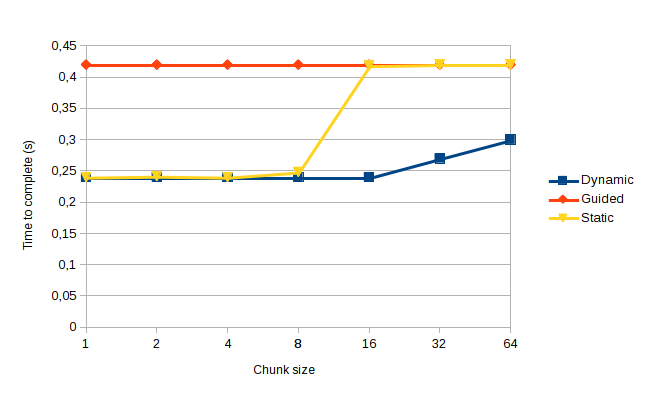
\includegraphics[width=0.8\textwidth]{loop1.png}
    \end{center}
    \caption{Run times for different schedulers and chunk sizes for the loop 1. The two schedulers without a specified chunk size, \texttt{auto} and \texttt{static} (with no size specified) achieved times of \(0,41s\) respectively.}
    \label{loop1}
\end{figure}

Looking at the code of the first loop reveals the sources of behaviour under different schedulers. The loop has most of its work at the beginning, which explains the constant time achieved with the \texttt{dynamic} scheduler and different chunk sizes. It also explains why the \texttt{static} scheduler is working fast with small chunk sizes, but starts to lag behind \texttt{dynamic} for larger ones - as the chunk size grows larger the amount of work in different threads gets more and more unbalanced, thus leading to the threads with less work to wait for the threads which had more work assigned to them. The \texttt{dynamic} scheduler wins for every chunk size, as the flexibility arising from each thread being able to pick up the next outstanding chunk apparently outweighs the communication costs.

\subsection{Second loop}
The results obtained for the second loop were much more varied. We can again readily notice the constant time for the \texttt{guided} scheduler, but there is a strong time minimum for both \texttt{static} and \texttt{dynamic} schedulers.

If we look carefully on how the number of iterations is assigned to the loop with iterator \textit{j}, we notice that when \textit{i} is less than 30, \textit{j} goes to N for every value of \textit{i}. When \(30 \leq i < 60\), only one in four \textit{j}s is assigned N iterations and the rest gets only one. In the following 30 only one in seven and so on (see line 73 in \texttt{loops.c}). Therefore the bulk of the computations is again at the beginning of the outermost loop, which explains the consistent behaviour of the \texttt{guided} scheduler. 

\begin{figure}[h!]
    \begin{center}
        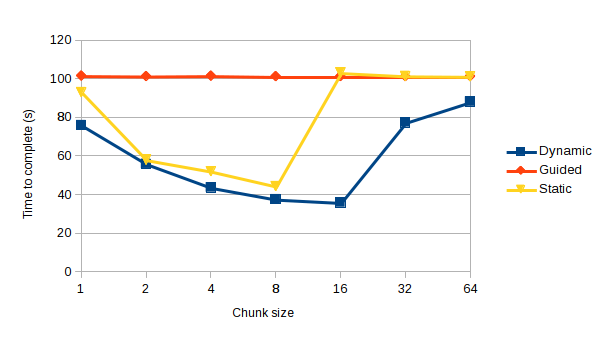
\includegraphics[width=0.8\textwidth]{loop2.png}
    \end{center}
    \caption{Run times for different schedulers and chunk sizes for the loop 2. For the \texttt{auto} and \texttt{static} without chunk size specified, we observe the execution times of \(99s\) and \(100s\), respectively.}
\end{figure}

Since the workload change period is 30, we would expect the most efficient scheduler to be one with a chunk size as close to 30 as possible, but that is not what happens. Instead we observe the time for both \texttt{static} and \texttt{dynamic} schedulers to decrease at first, but then drastically increase after the chunk size of 8 and 16 (respectively) is passed. 


\end{document}
